
%%%----------------------------------------------------------
%%%----------------------------------------------------------
%%%----------------------------------------------------------
%%%----------------------------------------------------------
%%%----------------------------------------------------------
\chapter{Door}
%%%----------------------------------------------------------

The activity "door" will be analyzed here with graphics.
%%%----------------------------------------------------------
\section{Test case 1}
%%%----------------------------------------------------------
Test case 1 in Fig.~\ref{fig:Test_case_door_1}
\begin{figure}
	\centering\small
	\setlength{\tabcolsep}{0mm}	% alle Spaltenränder auf 0mm
	\begin{tabular}{c@{\hspace{12mm}}c} % mittlerer Abstand = 12mm
		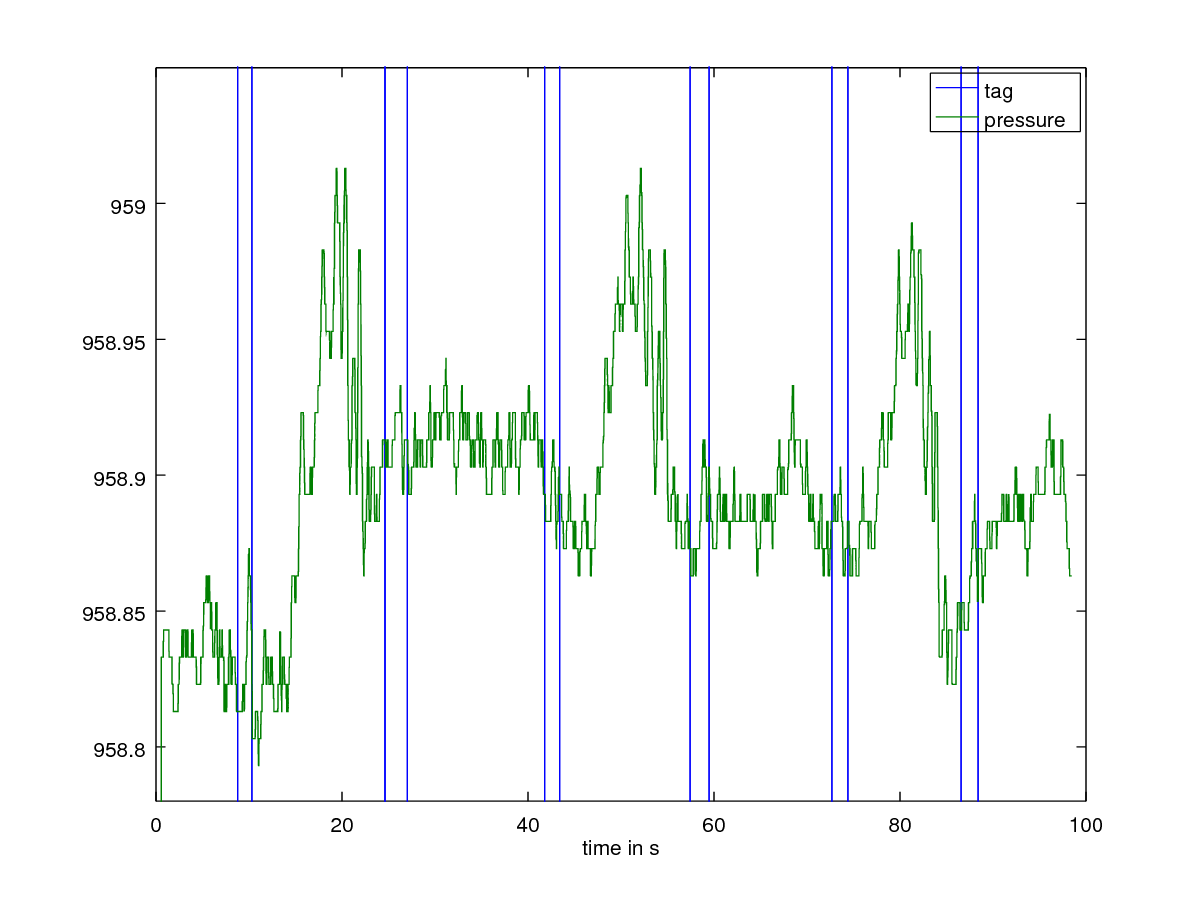
\includegraphics[width=.45\textwidth]{doormultiplenewnew3_p} &
		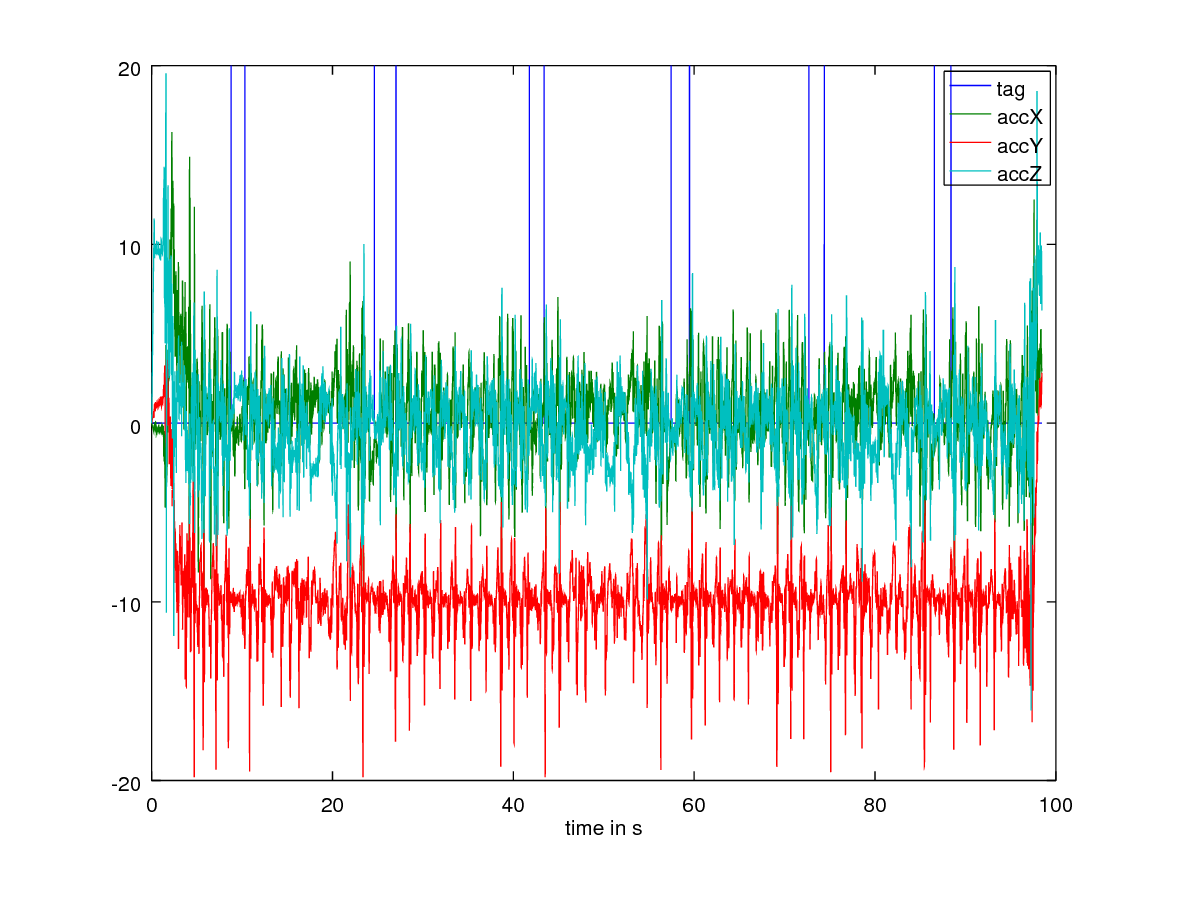
\includegraphics[width=.45\textwidth]{doormultiplenewnew3_a} 
		\\
		(a) & (b)
		\\[4pt]	%vertical extra spacing (4 points)
		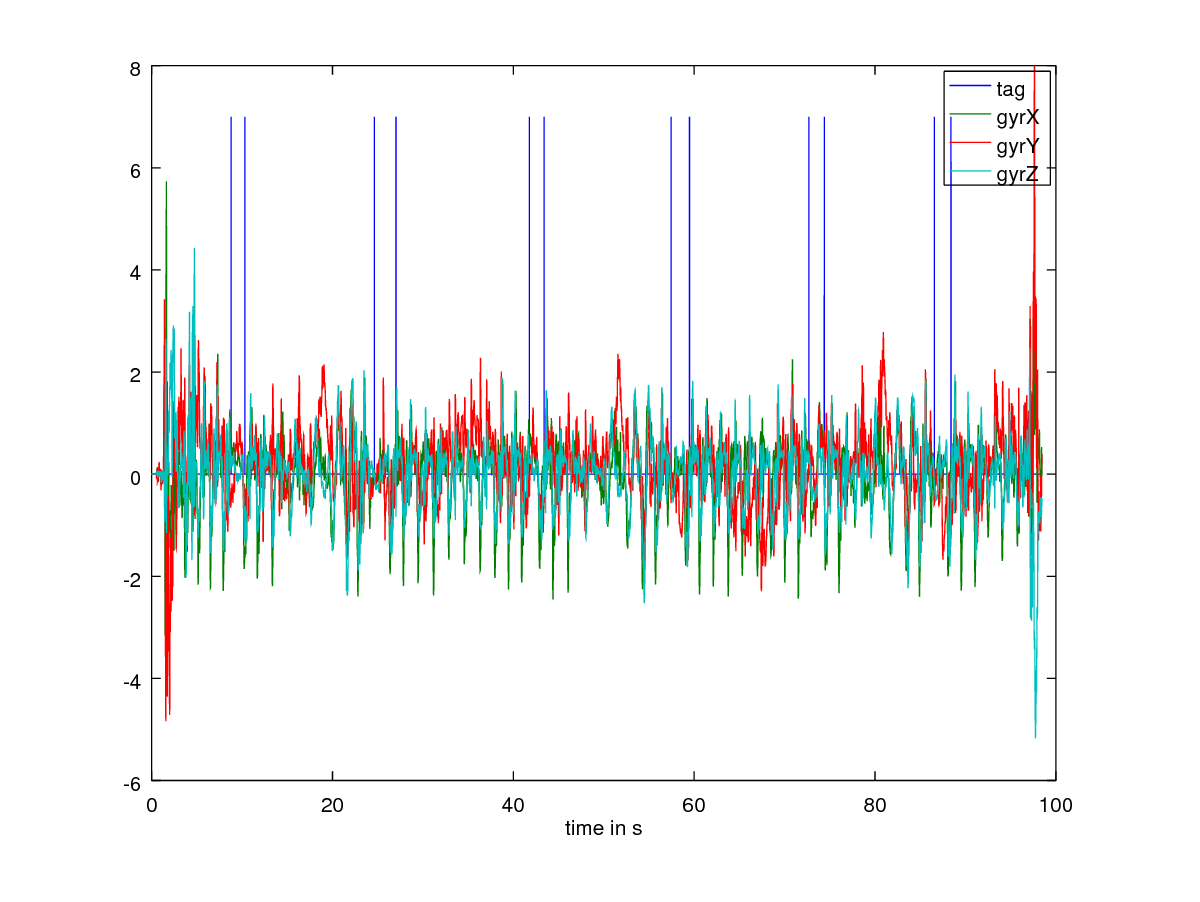
\includegraphics[width=.45\textwidth]{doormultiplenewnew3_g} &
		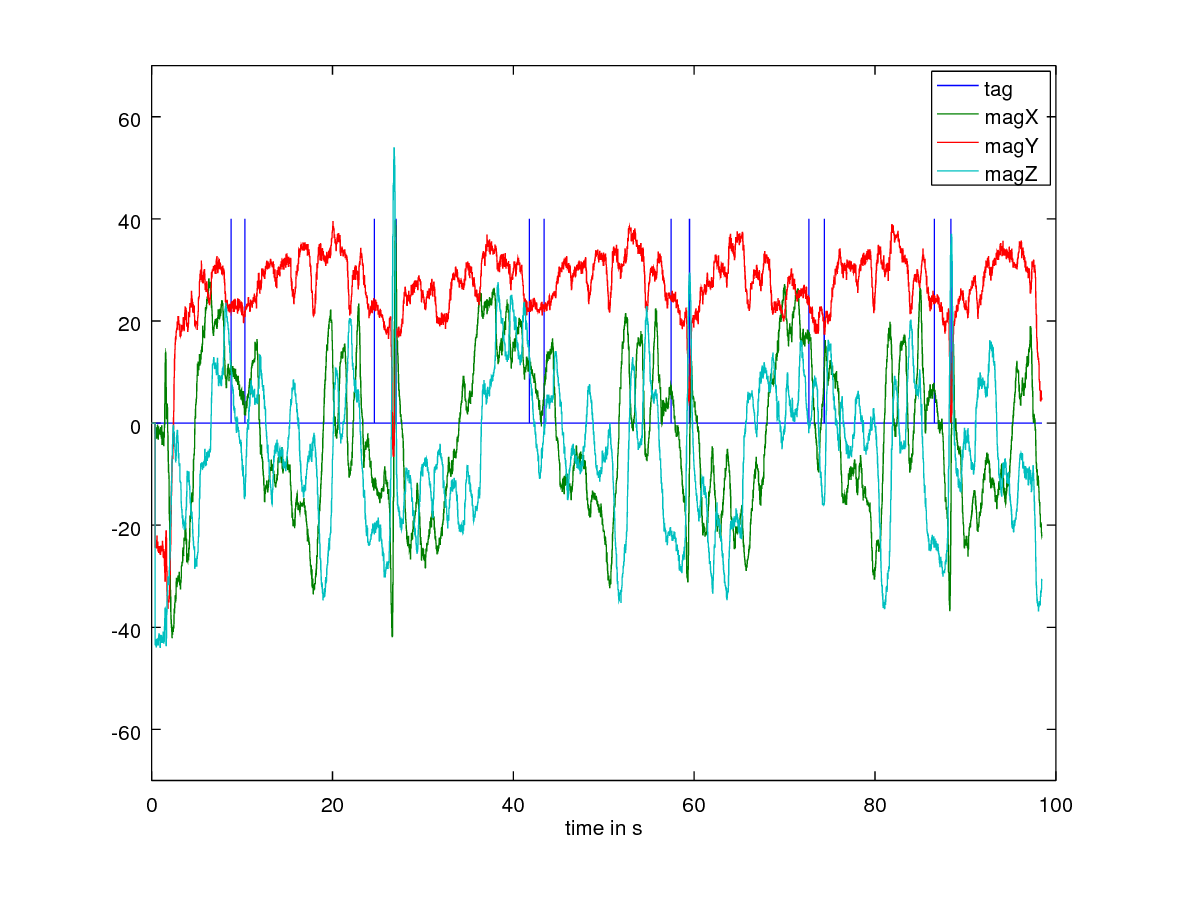
\includegraphics[width=.45\textwidth]{doormultiplenewnew3_m} 
		\\
		(c) & (d)
		\\[4pt]	%vertical extra spacing (4 points)
		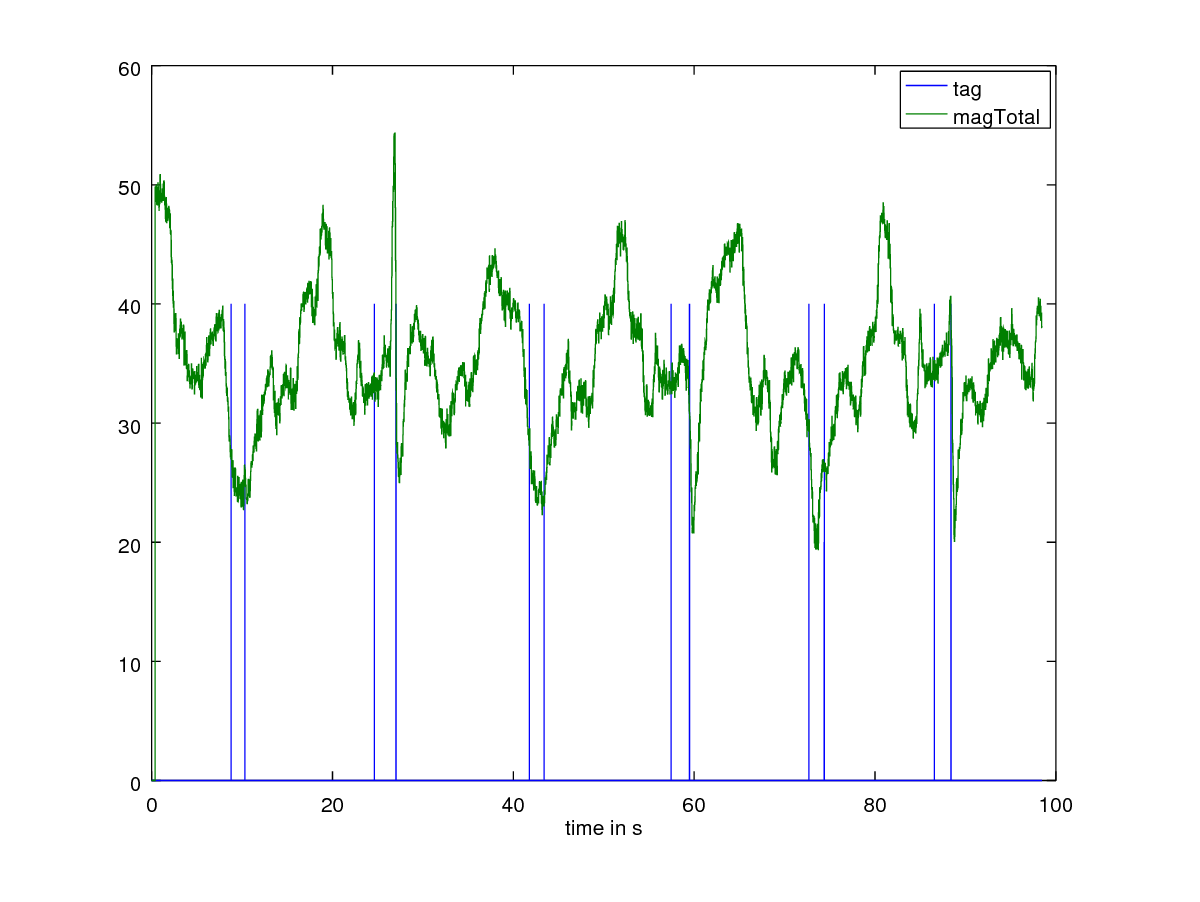
\includegraphics[width=.45\textwidth]{doormultiplenewnew3_mtotal} 
		\\
		(e) 
	\end{tabular}
	%
	\caption{Test case 1}
	\label{fig:Test_case_door_1}
\end{figure}

%%%----------------------------------------------------------
\section{Test case 1.1}
%%%----------------------------------------------------------
Test case 1.1 in Fig.~\ref{fig:Test_case_door_1_1}
\begin{figure}
	\centering\small
	\setlength{\tabcolsep}{0mm}	% alle Spaltenränder auf 0mm
	\begin{tabular}{c@{\hspace{12mm}}c} % mittlerer Abstand = 12mm
		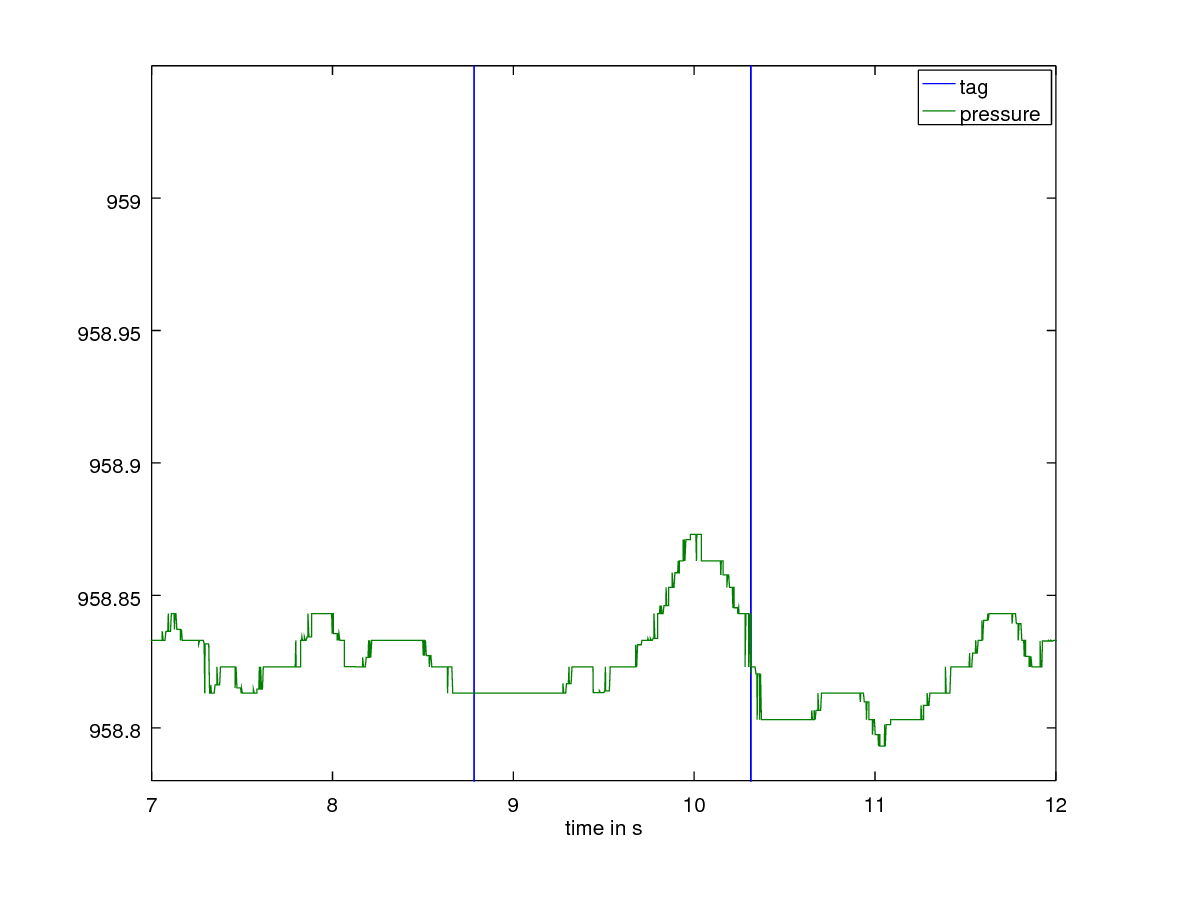
\includegraphics[width=.45\textwidth]{doormultiplenewnew3_1_p} &
		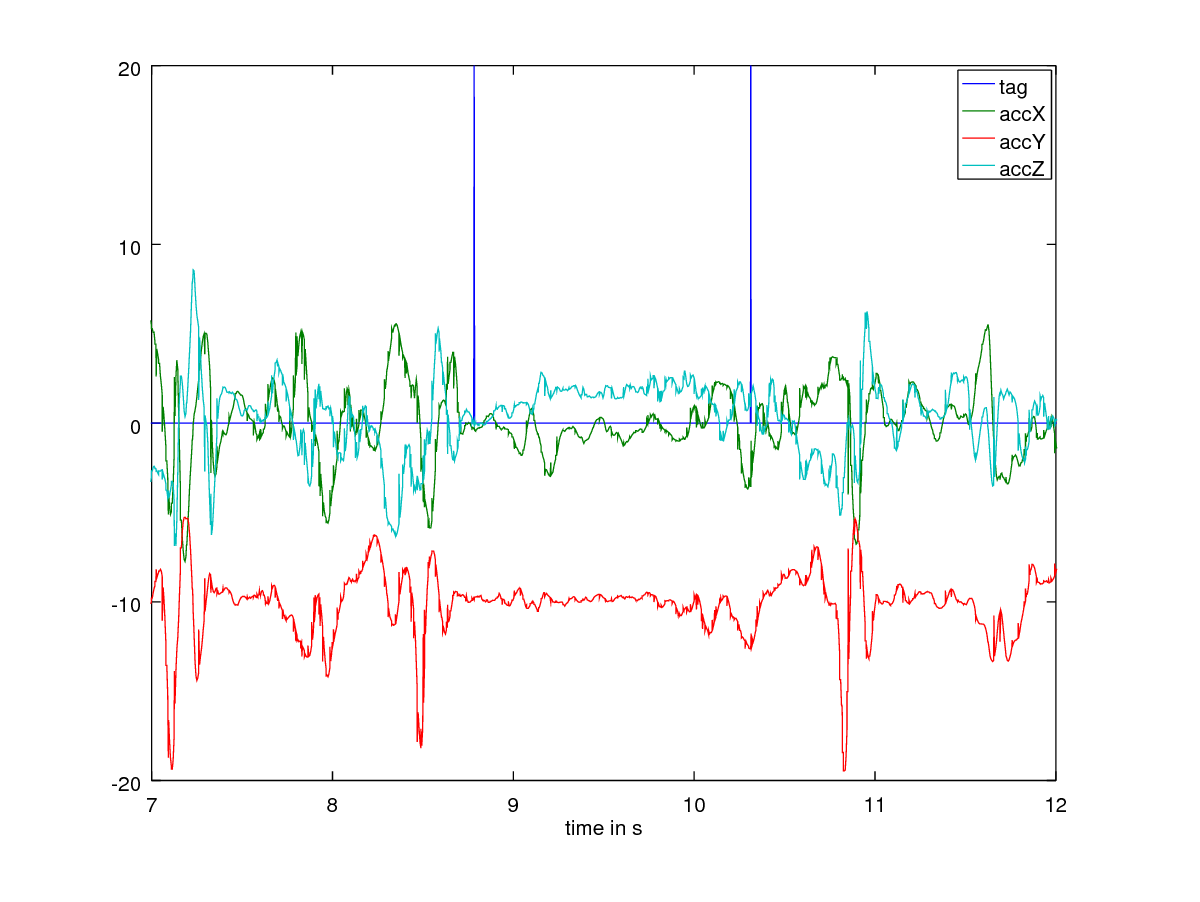
\includegraphics[width=.45\textwidth]{doormultiplenewnew3_1_a} 
		\\
		(a) & (b)
		\\[4pt]	%vertical extra spacing (4 points)
		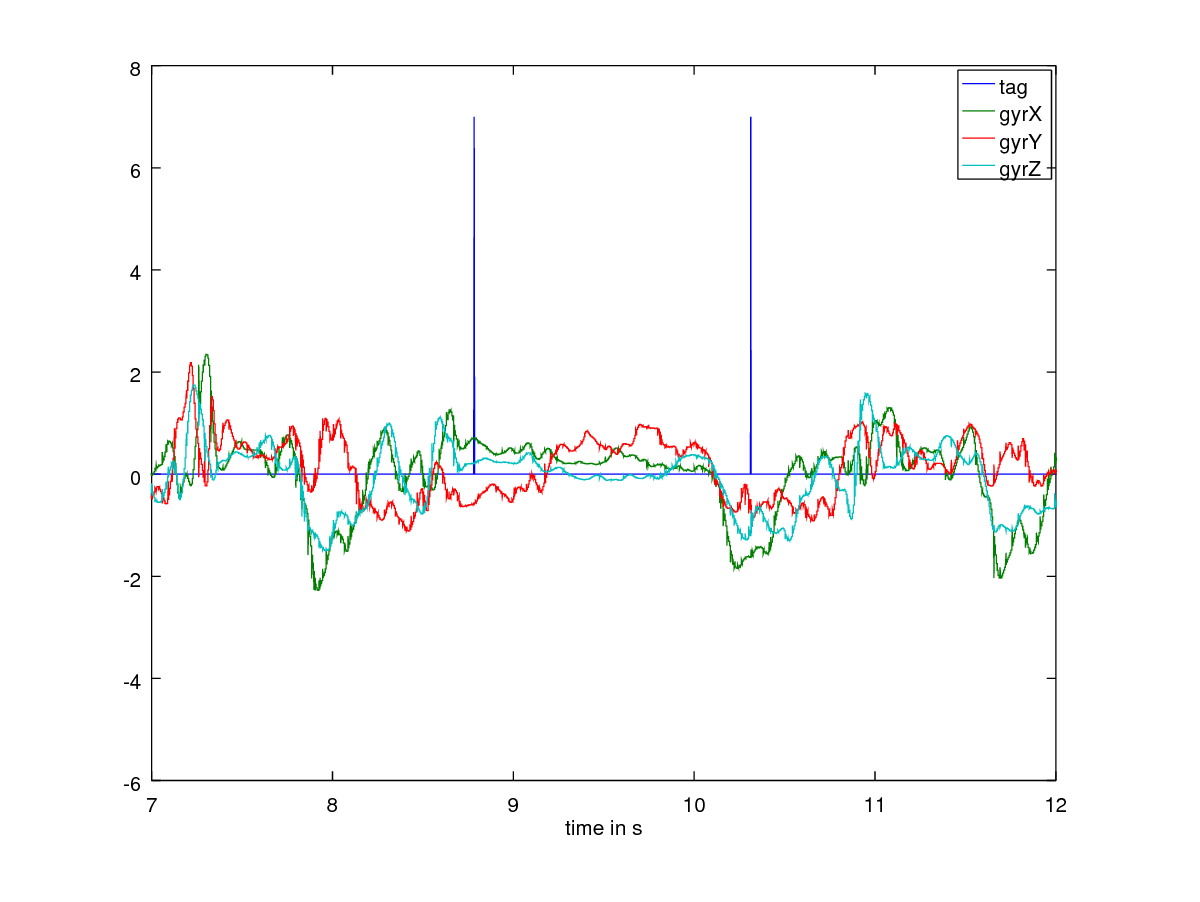
\includegraphics[width=.45\textwidth]{doormultiplenewnew3_1_g} &
		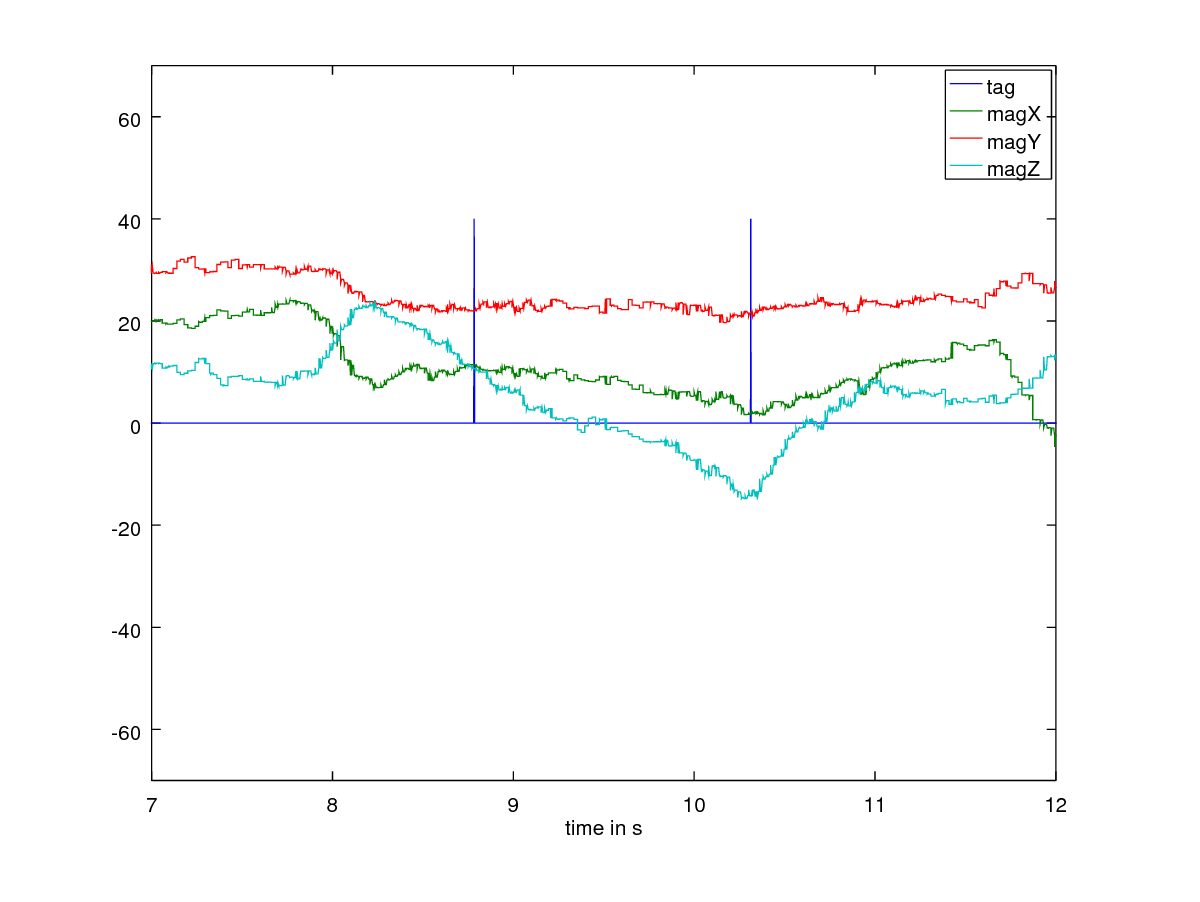
\includegraphics[width=.45\textwidth]{doormultiplenewnew3_1_m} 
		\\
		(c) & (d)
		\\[4pt]	%vertical extra spacing (4 points)
		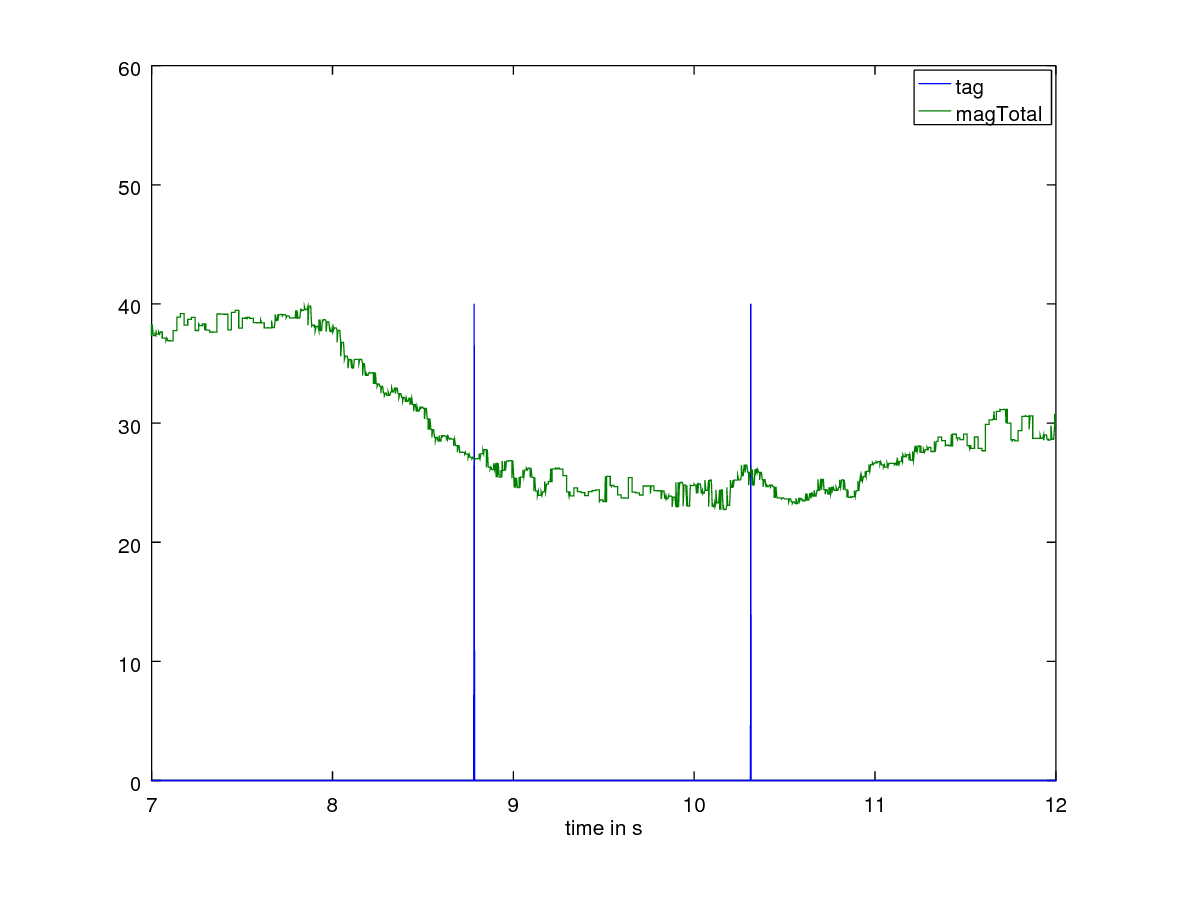
\includegraphics[width=.45\textwidth]{doormultiplenewnew3_1_mtotal} 
		\\
		(e) 
	\end{tabular}
	%
	\caption{Test case 1.1}
	\label{fig:Test_case_door_1_1}
\end{figure}

%%%----------------------------------------------------------
\section{Test case 2}
%%%----------------------------------------------------------

Test case 2 in Fig.~\ref{fig:Test_case_door_2}
\begin{figure}
	\centering\small
	\setlength{\tabcolsep}{0mm}	% alle Spaltenränder auf 0mm
	\begin{tabular}{c@{\hspace{12mm}}c} % mittlerer Abstand = 12mm
		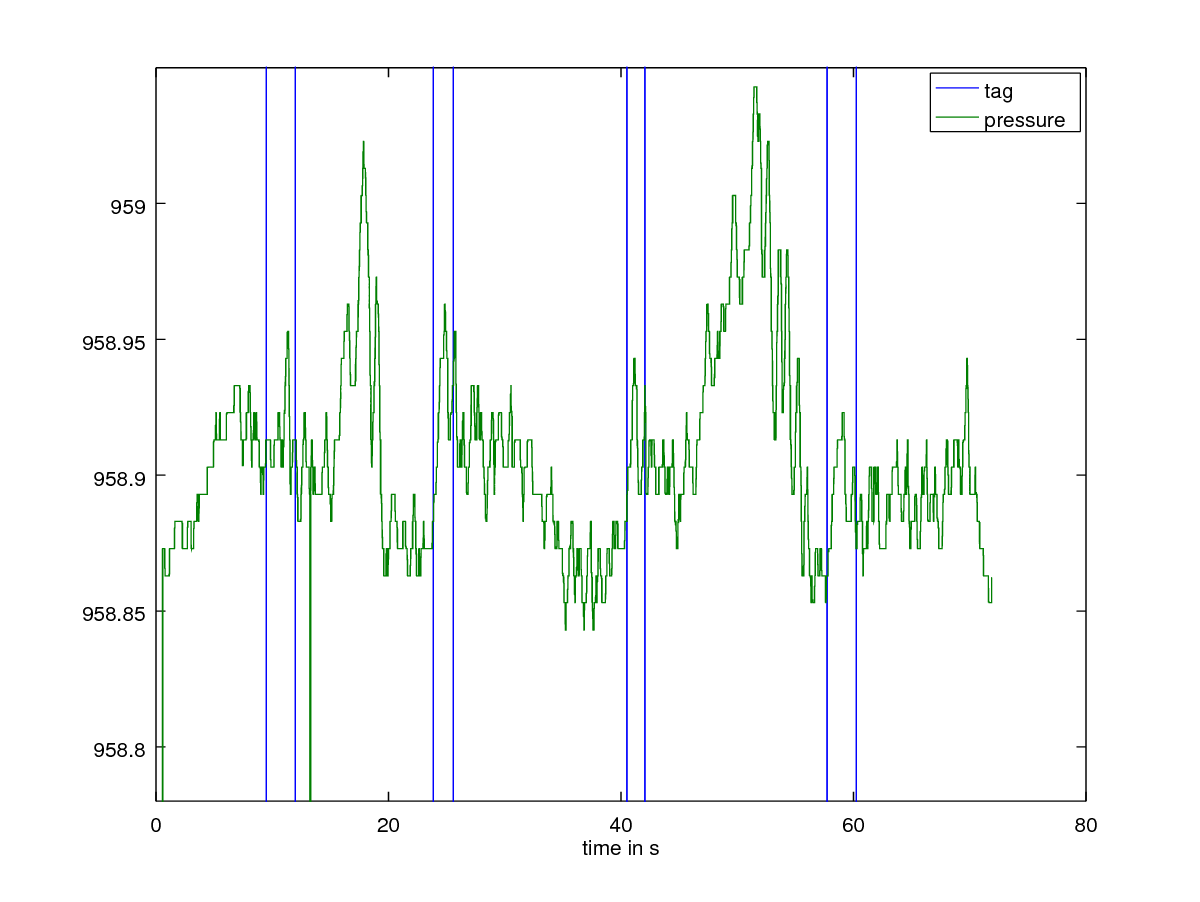
\includegraphics[width=.45\textwidth]{doorwendelmultiple_p} &
		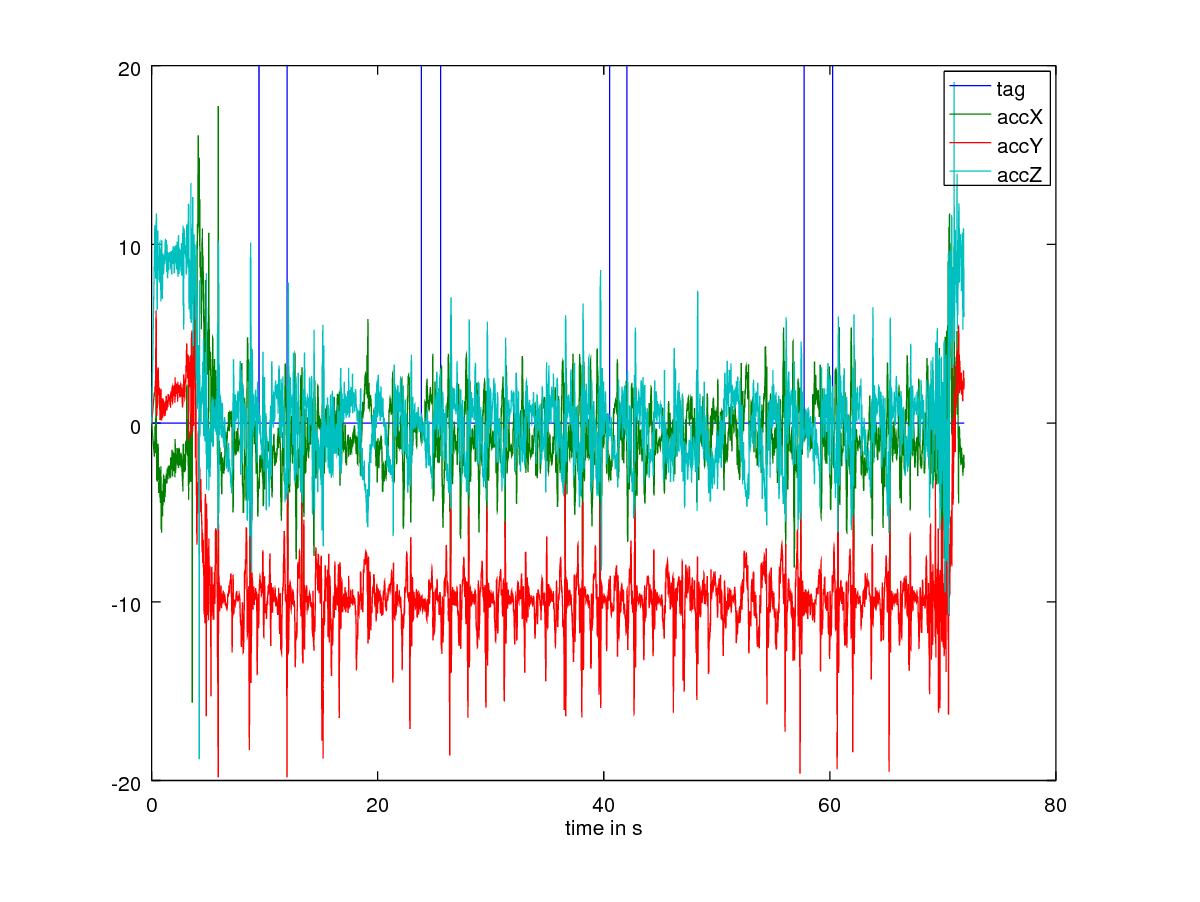
\includegraphics[width=.45\textwidth]{doorwendelmultiple_a} 
		\\
		(a) & (b)
		\\[4pt]	%vertical extra spacing (4 points)
		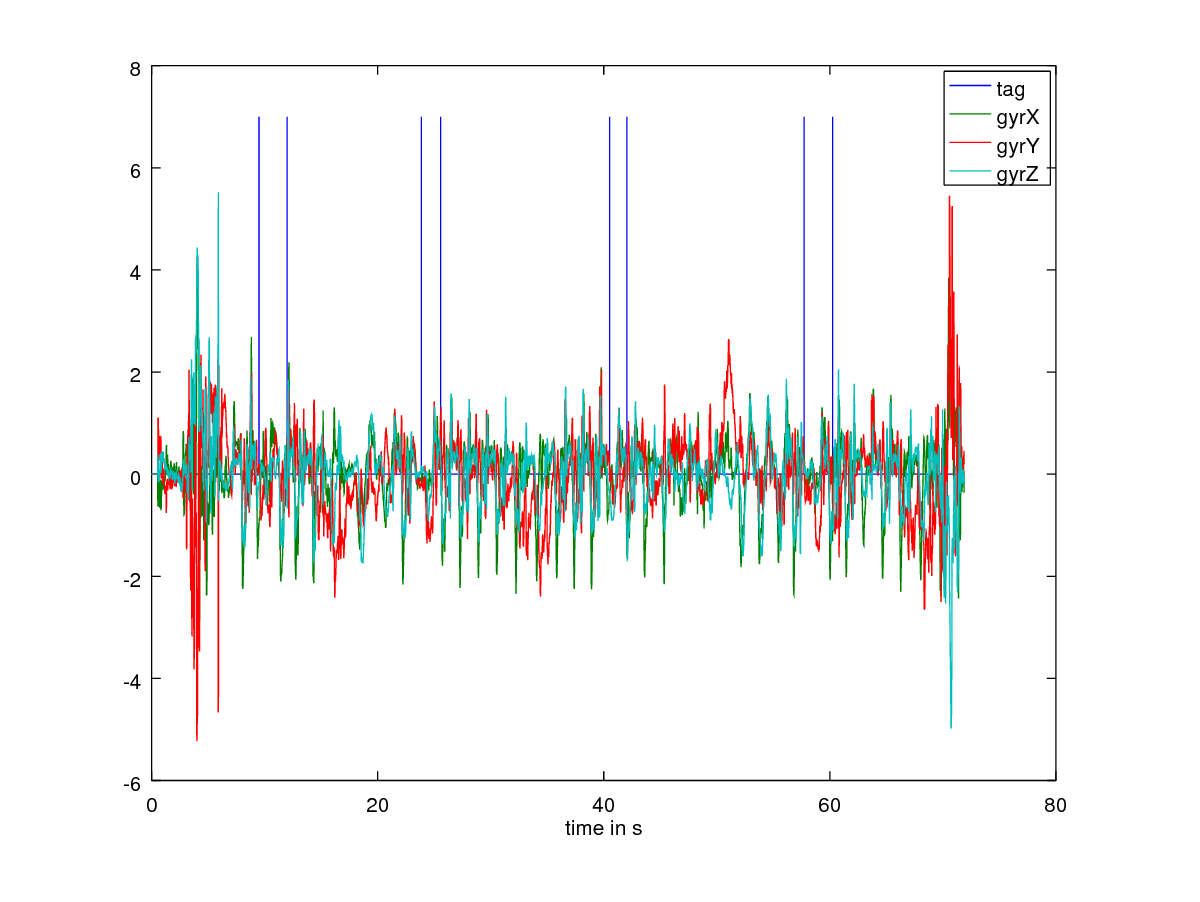
\includegraphics[width=.45\textwidth]{doorwendelmultiple_g} &
		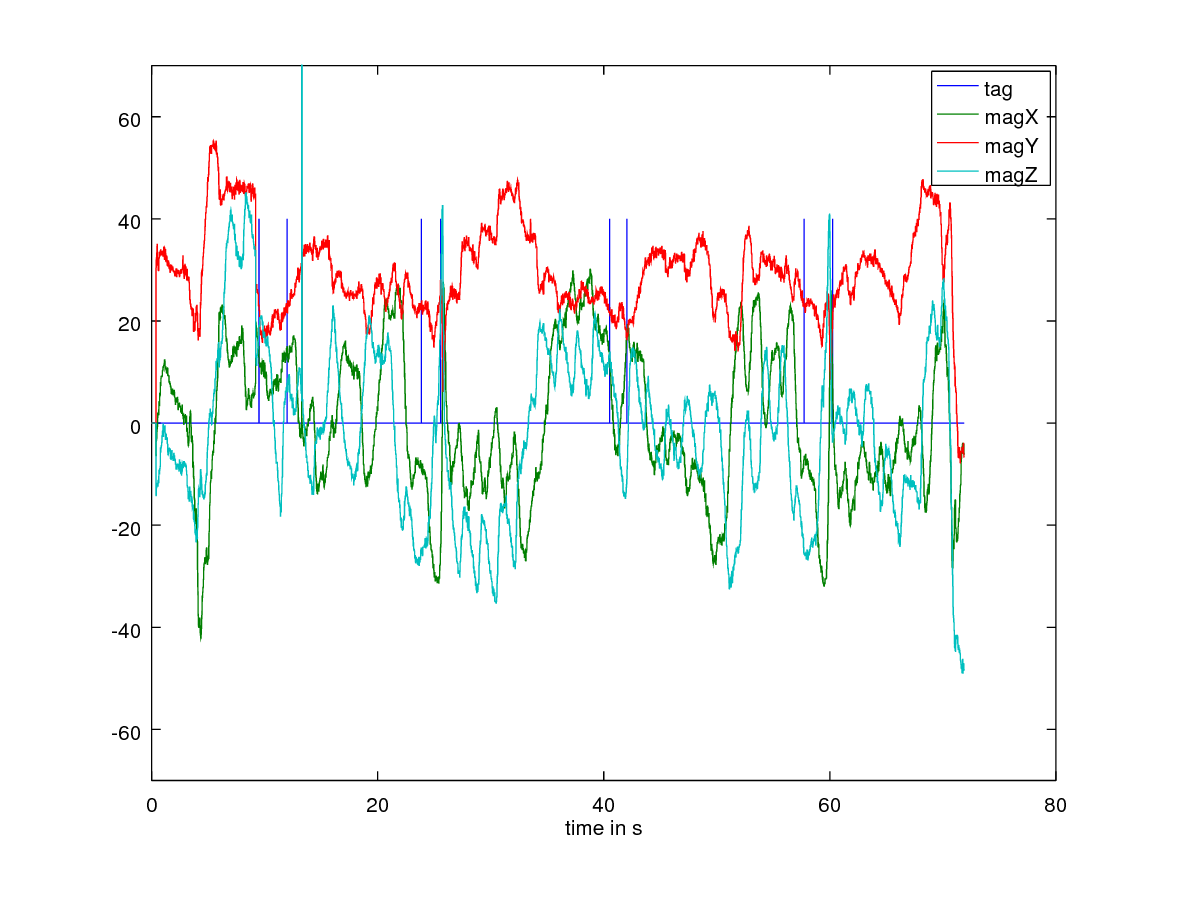
\includegraphics[width=.45\textwidth]{doorwendelmultiple_m} 
		\\
		(c) & (d)
		\\[4pt]	%vertical extra spacing (4 points)
		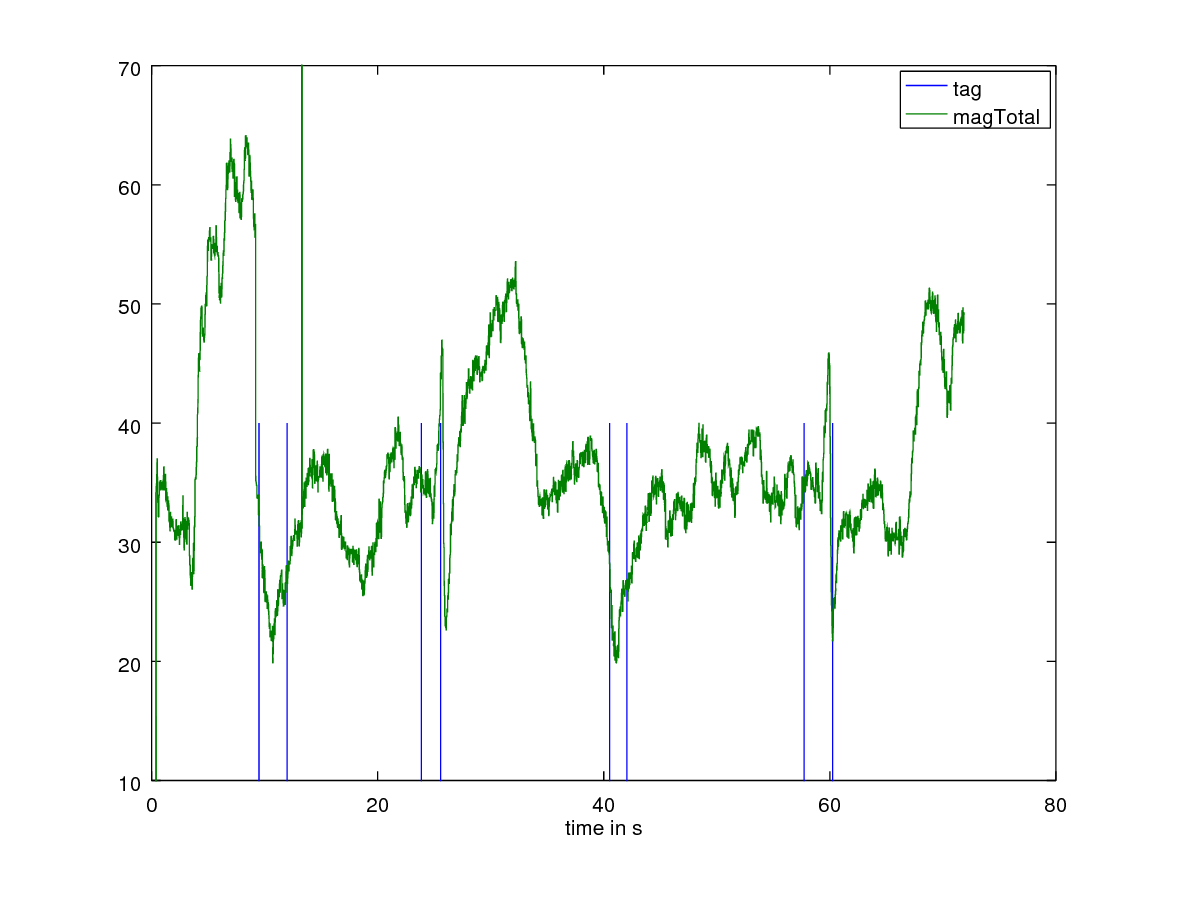
\includegraphics[width=.45\textwidth]{doorwendelmultiple_mtotal} 
		\\
		(e) 
	\end{tabular}
	%
	\caption{Test case 2}
	\label{fig:Test_case_door_2}
\end{figure}


%%%----------------------------------------------------------
\section{Test case 3}
%%%----------------------------------------------------------
Test case 3 in Fig.~\ref{fig:Test_case_door_3}
\begin{figure}
	\centering\small
	\setlength{\tabcolsep}{0mm}	% alle Spaltenränder auf 0mm
	\begin{tabular}{c@{\hspace{12mm}}c} % mittlerer Abstand = 12mm
		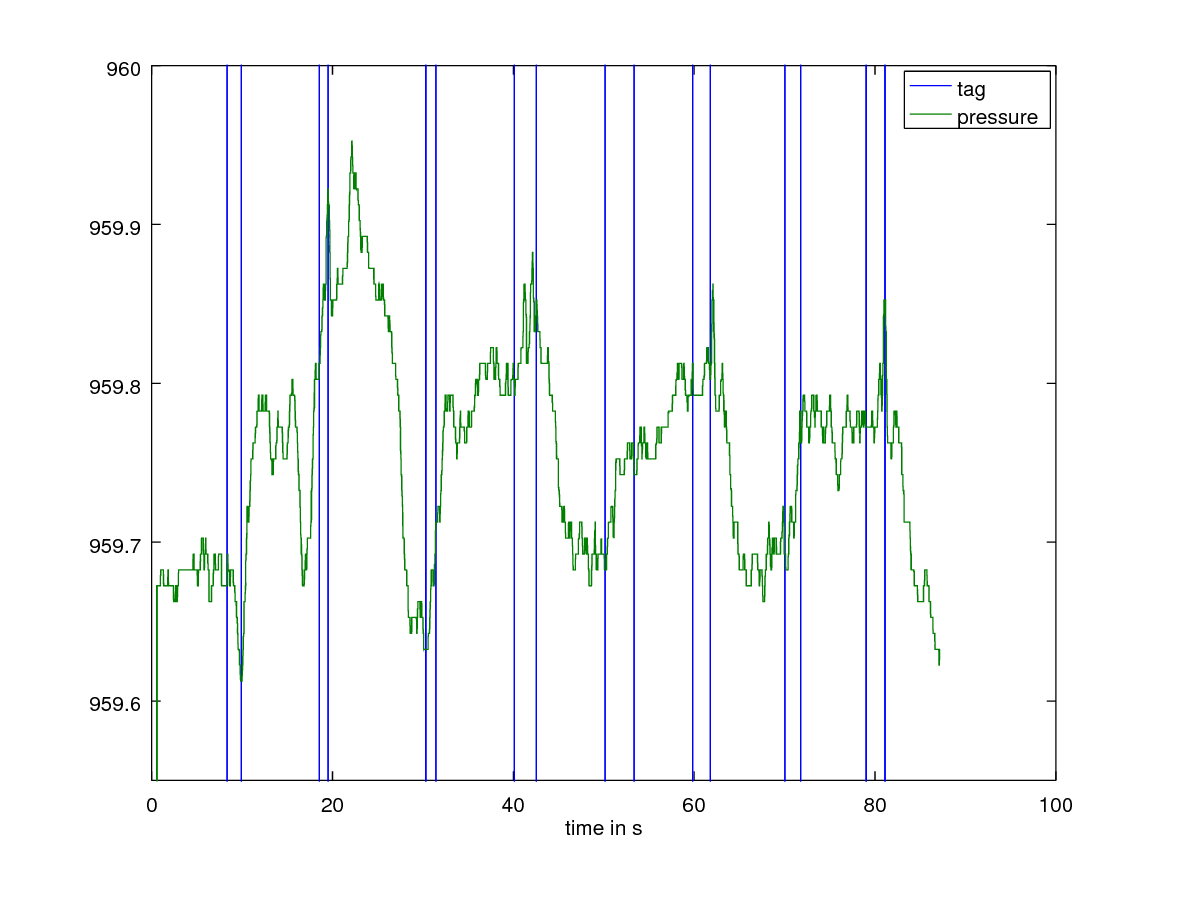
\includegraphics[width=.45\textwidth]{pubdoormult6678_p} &
		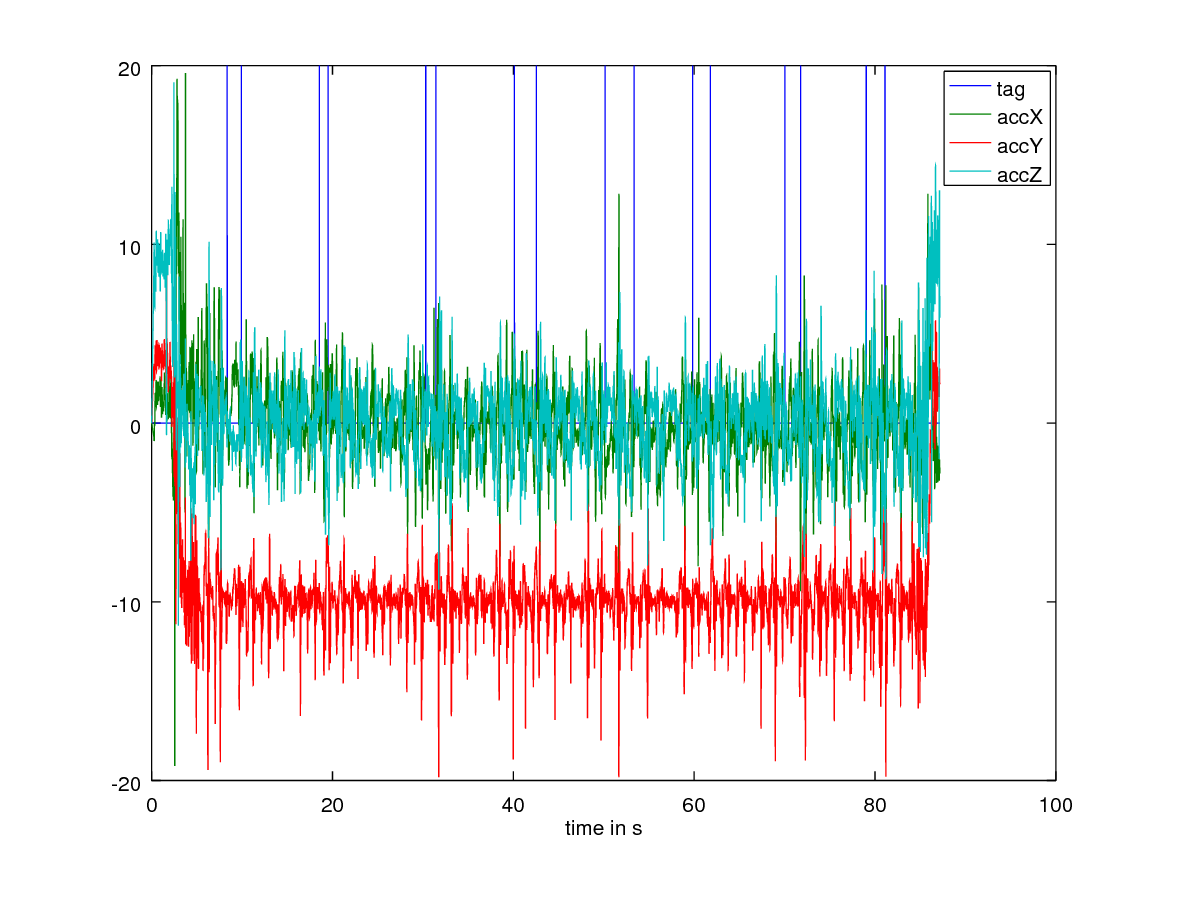
\includegraphics[width=.45\textwidth]{pubdoormult6678_a} 
		\\
		(a) & (b)
		\\[4pt]	%vertical extra spacing (4 points)
		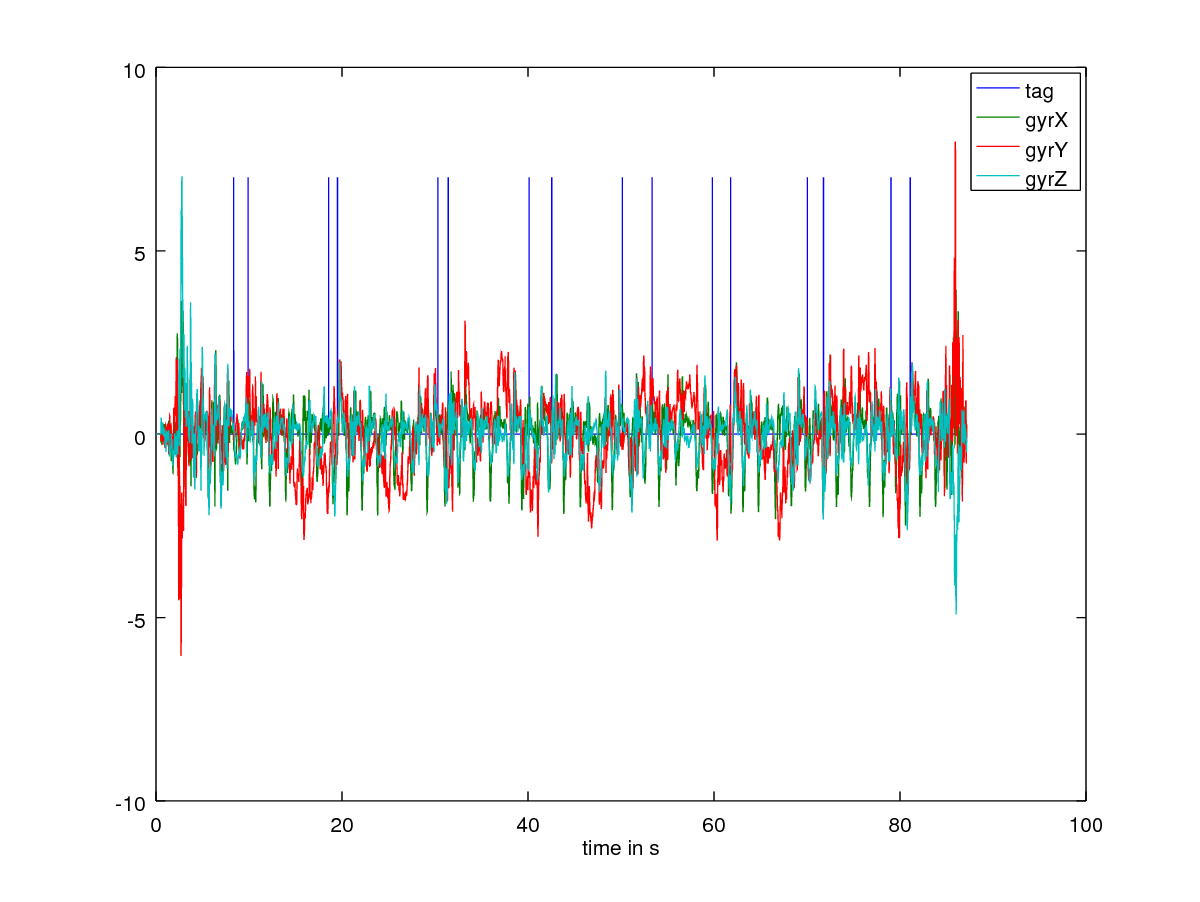
\includegraphics[width=.45\textwidth]{pubdoormult6678_g} &
		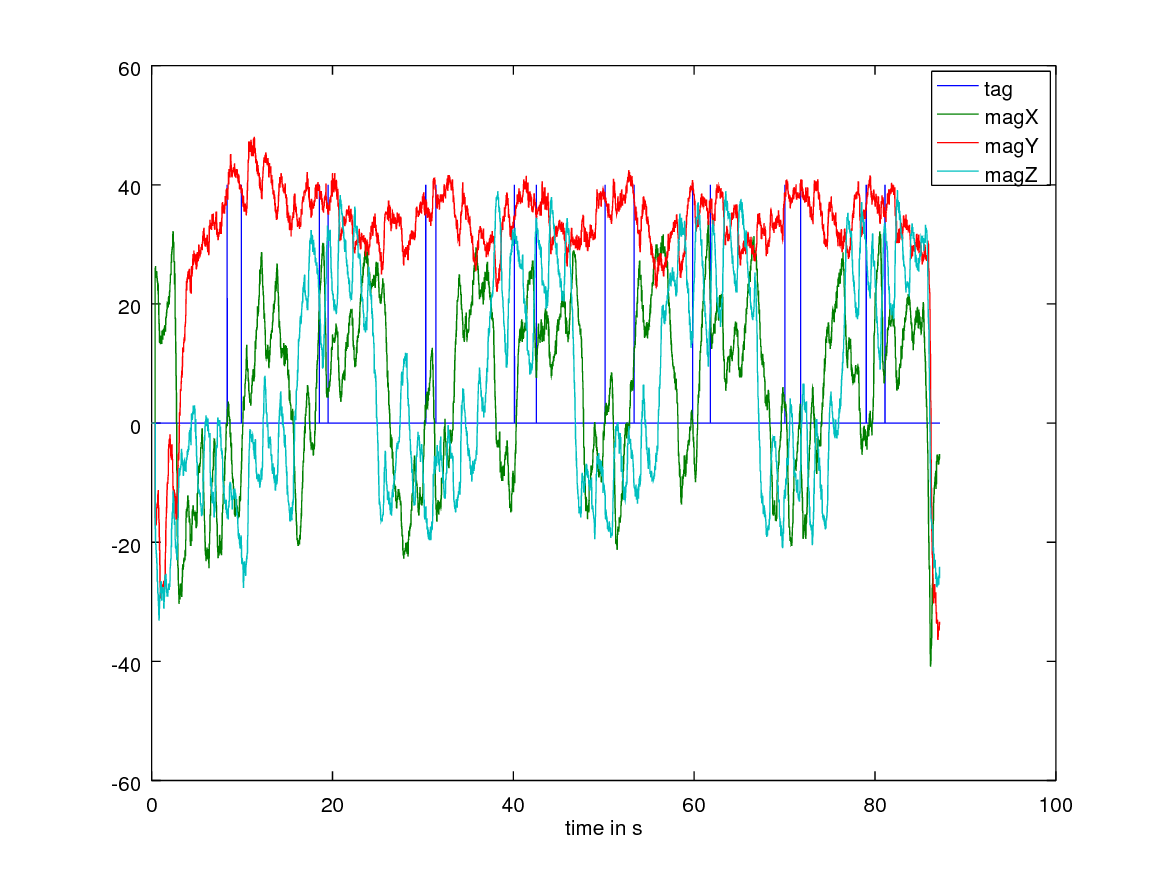
\includegraphics[width=.45\textwidth]{pubdoormult6678_m} 
		\\
		(c) & (d)
		\\[4pt]	%vertical extra spacing (4 points)
		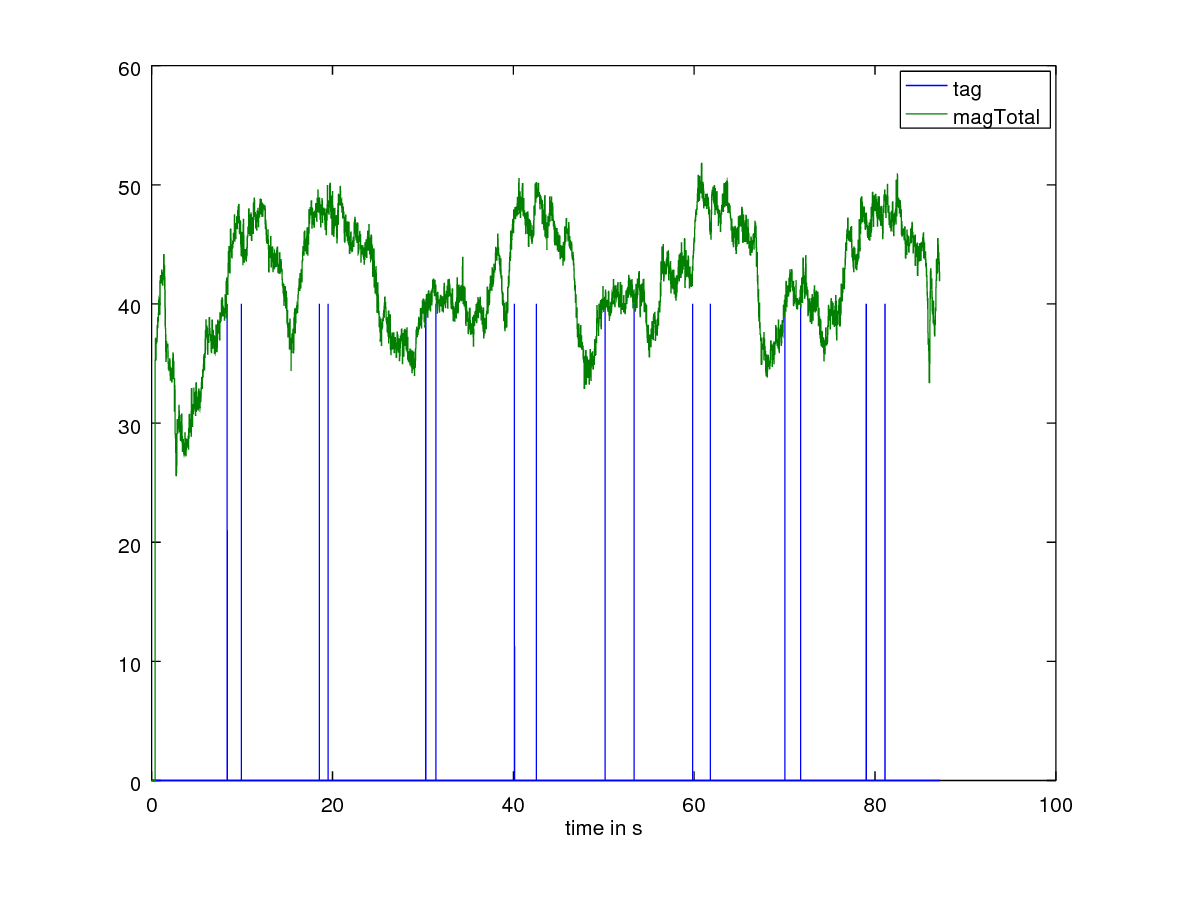
\includegraphics[width=.45\textwidth]{pubdoormult6678_mtotal}  
		\\
		(e)
	\end{tabular}
	%
	\caption{Test case 3}
	\label{fig:Test_case_door_3}
\end{figure}

%%%----------------------------------------------------------
\section{Test case 4}
%%%----------------------------------------------------------
Test case 4 in Fig.~\ref{fig:Test_case_door_4}
\begin{figure}
	\centering\small
	\setlength{\tabcolsep}{0mm}	% alle Spaltenränder auf 0mm
	\begin{tabular}{c@{\hspace{12mm}}c} % mittlerer Abstand = 12mm
		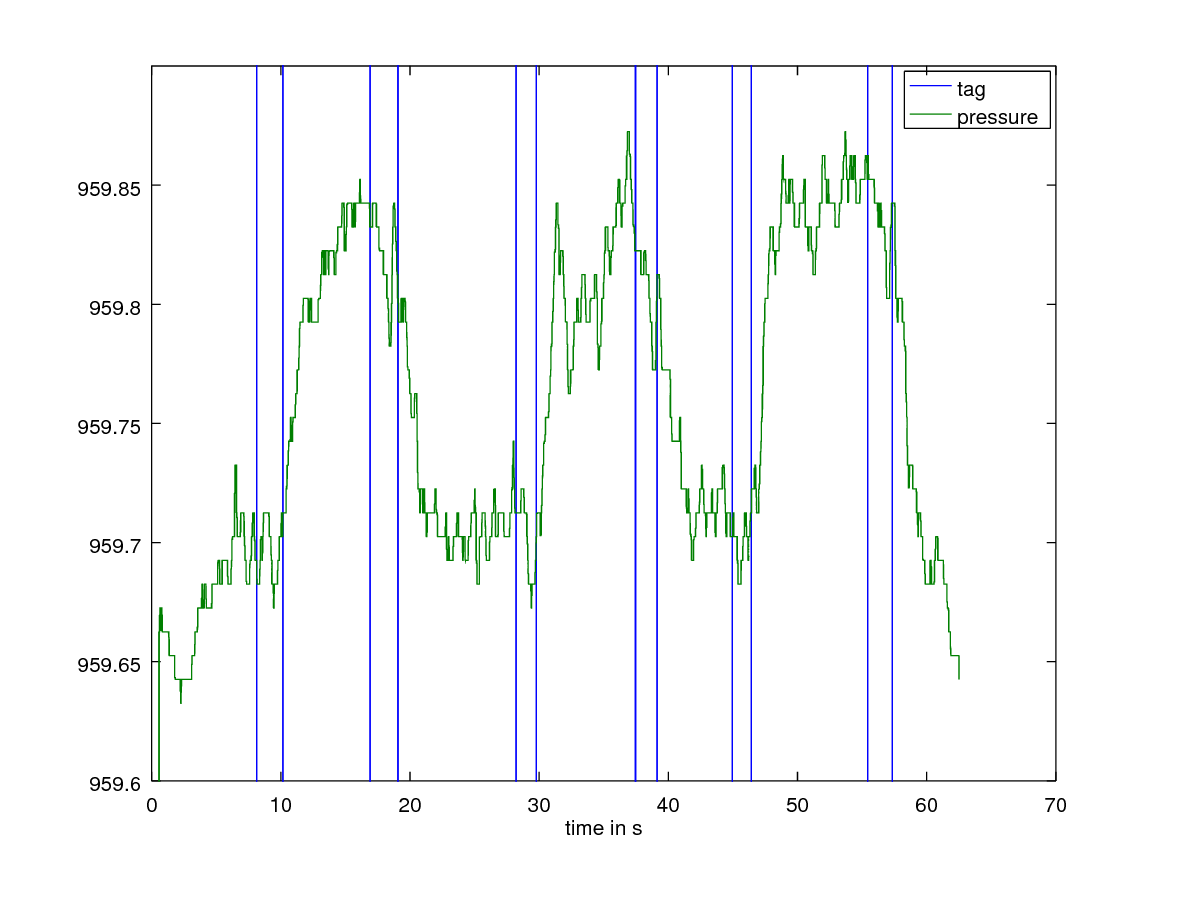
\includegraphics[width=.45\textwidth]{pubdoormult_p} &
		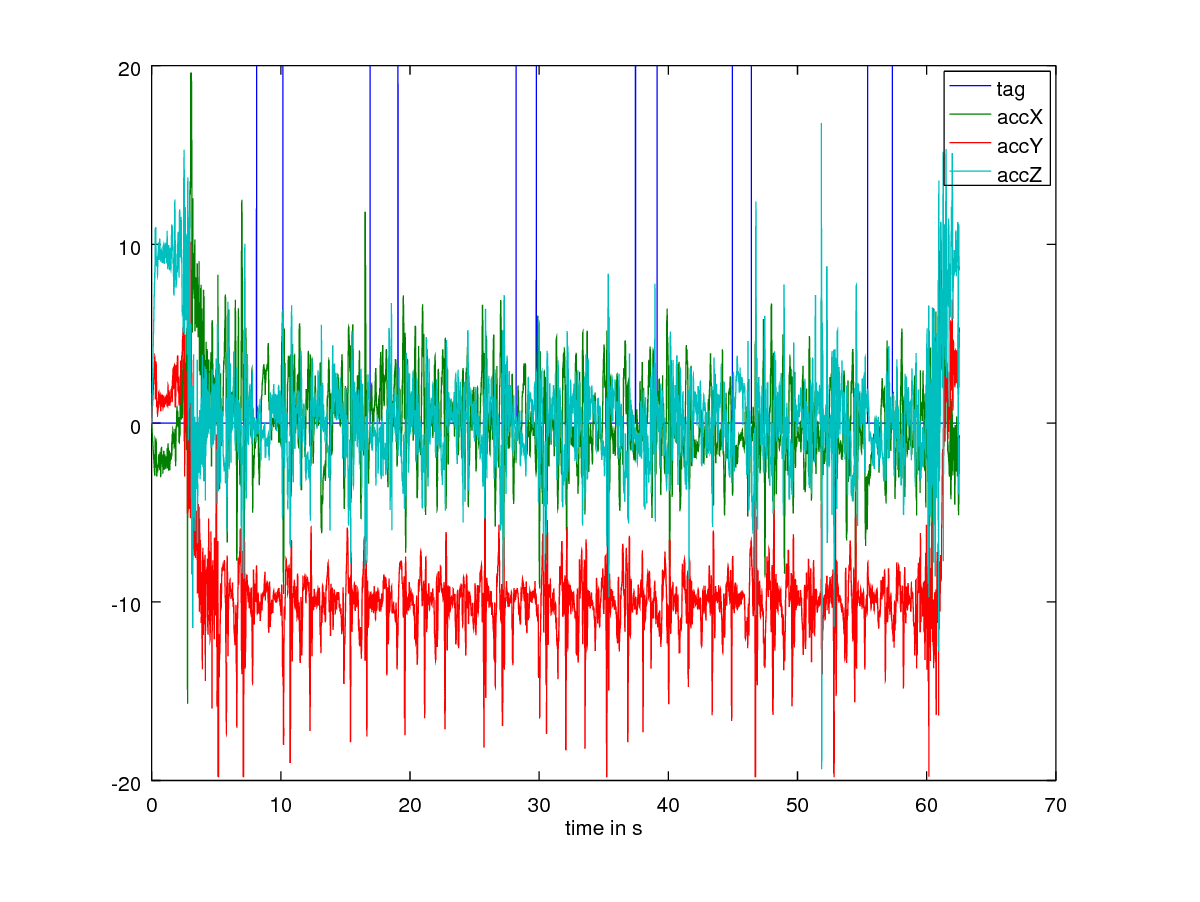
\includegraphics[width=.45\textwidth]{pubdoormult_a} 
		\\
		(a) & (b)
		\\[4pt]	%vertical extra spacing (4 points)
		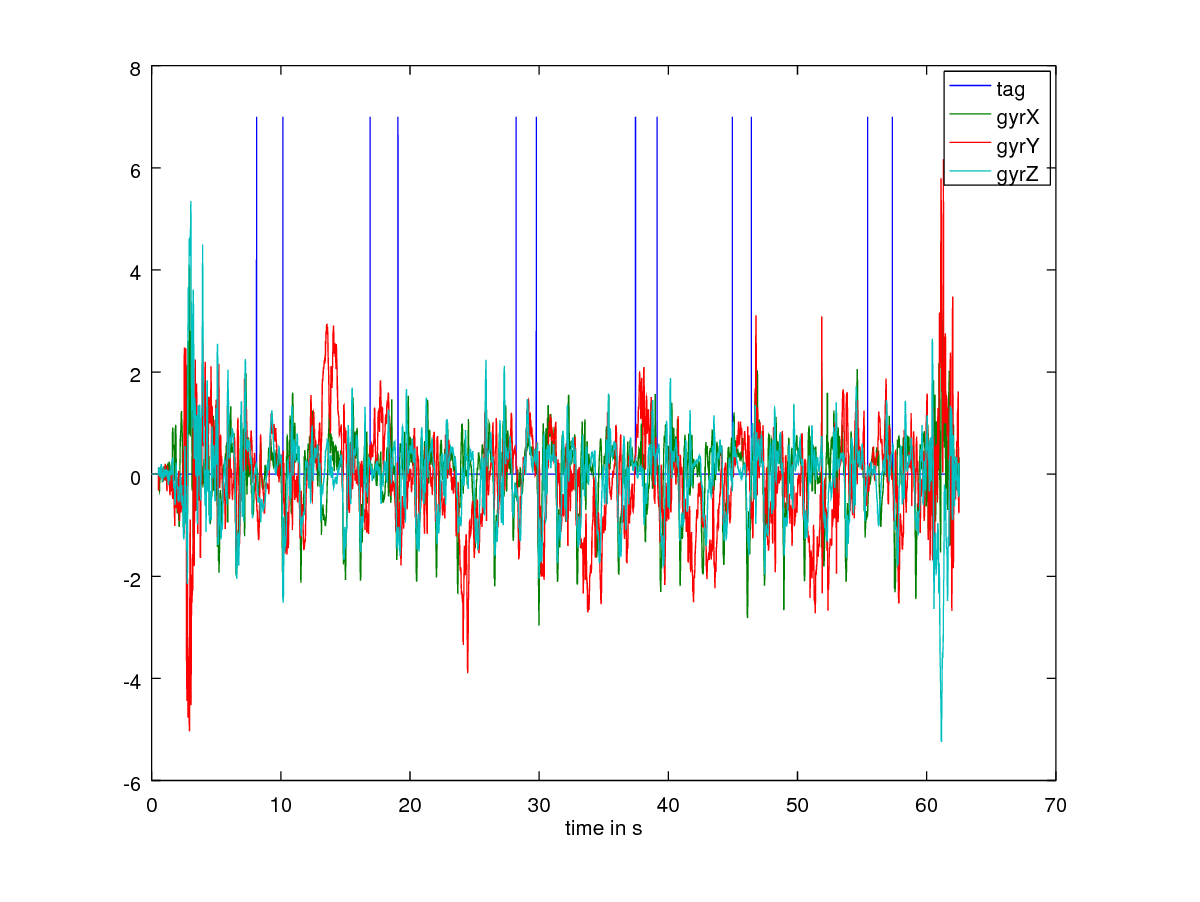
\includegraphics[width=.45\textwidth]{pubdoormult_g} &
		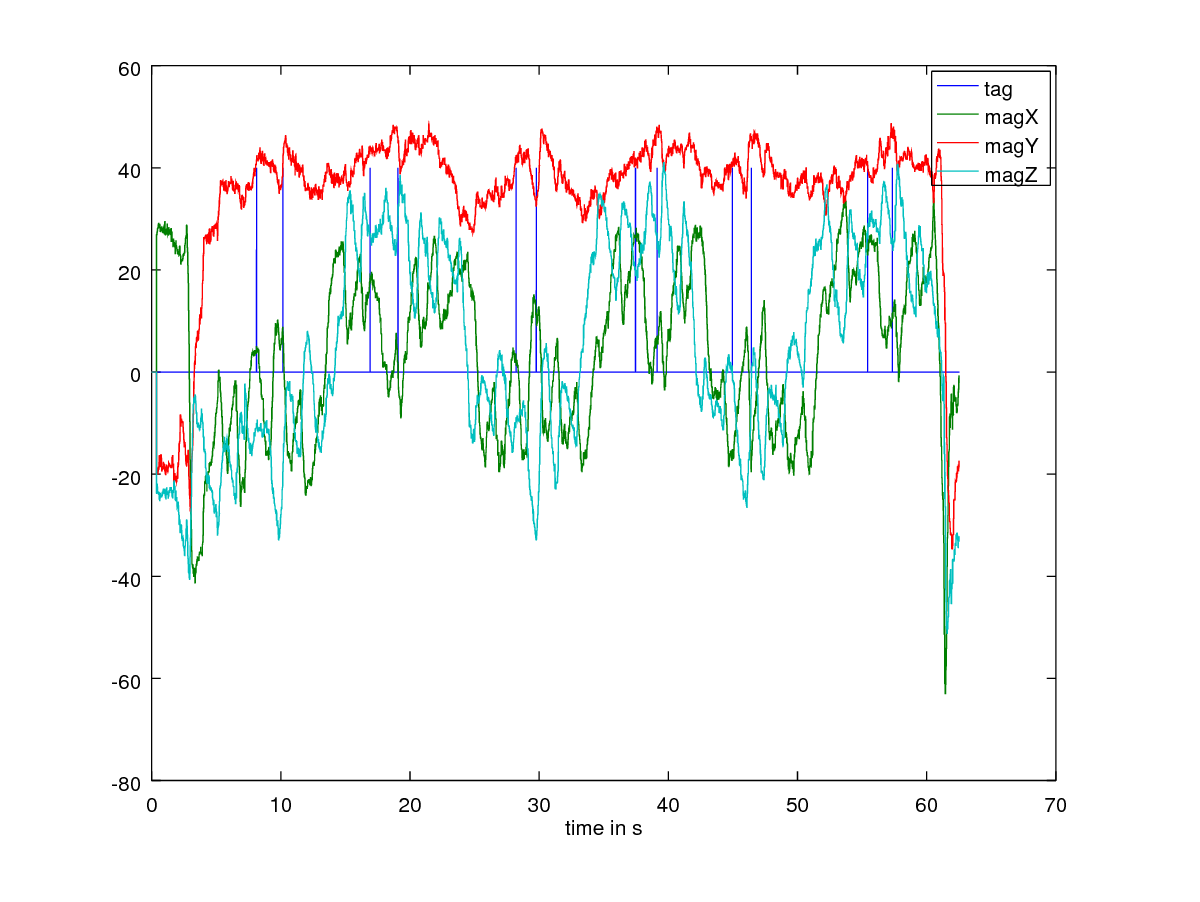
\includegraphics[width=.45\textwidth]{pubdoormult_m} 
		\\
		(c) & (d)
		\\[4pt]	%vertical extra spacing (4 points)
		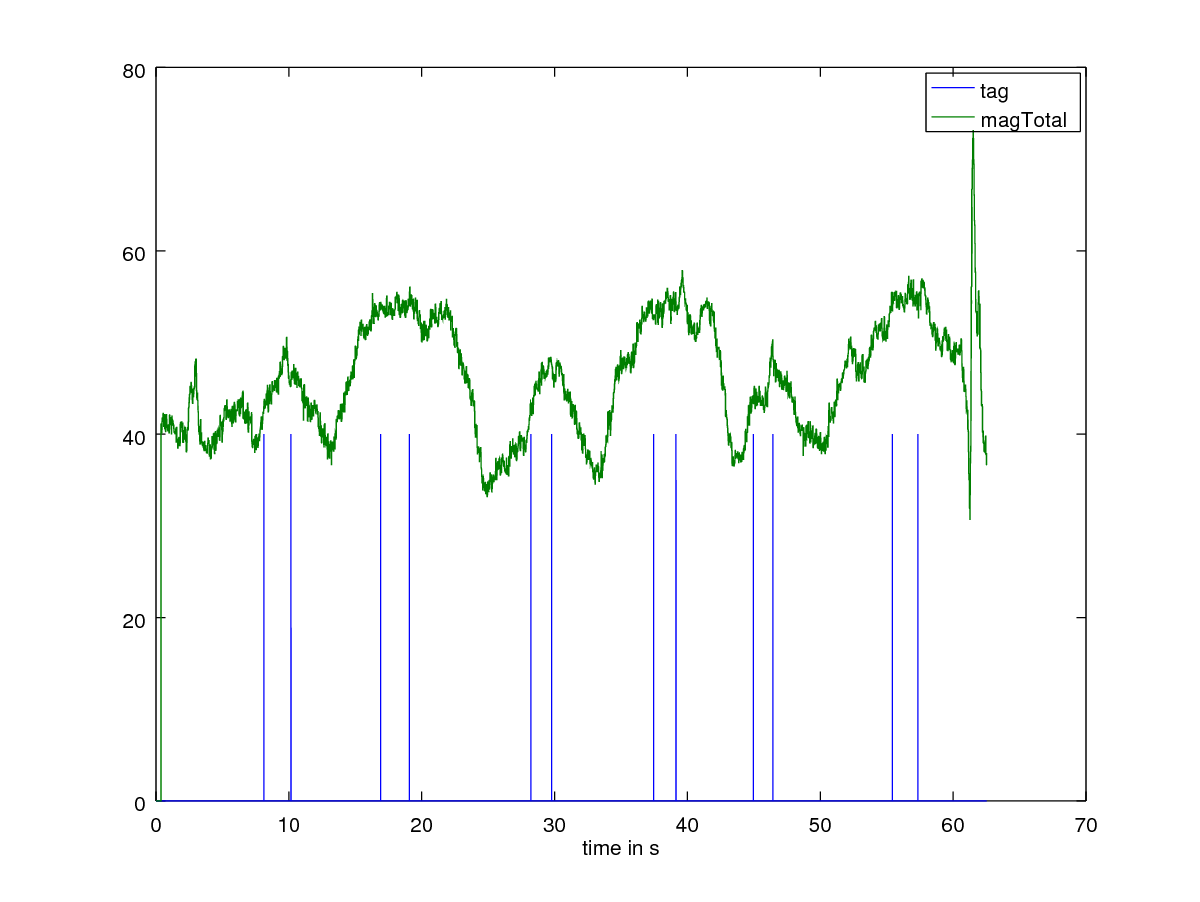
\includegraphics[width=.45\textwidth]{pubdoormult_mtotal} 
		\\
		(e)
	\end{tabular}
	%
	\caption{Test case 4}
	\label{fig:Test_case_door_4}
\end{figure}

%%%----------------------------------------------------------
\section{Test case 5}
%%%----------------------------------------------------------
Test case 5 in Fig.~\ref{fig:Test_case_door_5}
\begin{figure}
	\centering\small
	\setlength{\tabcolsep}{0mm}	% alle Spaltenränder auf 0mm
	\begin{tabular}{c@{\hspace{12mm}}c} % mittlerer Abstand = 12mm
		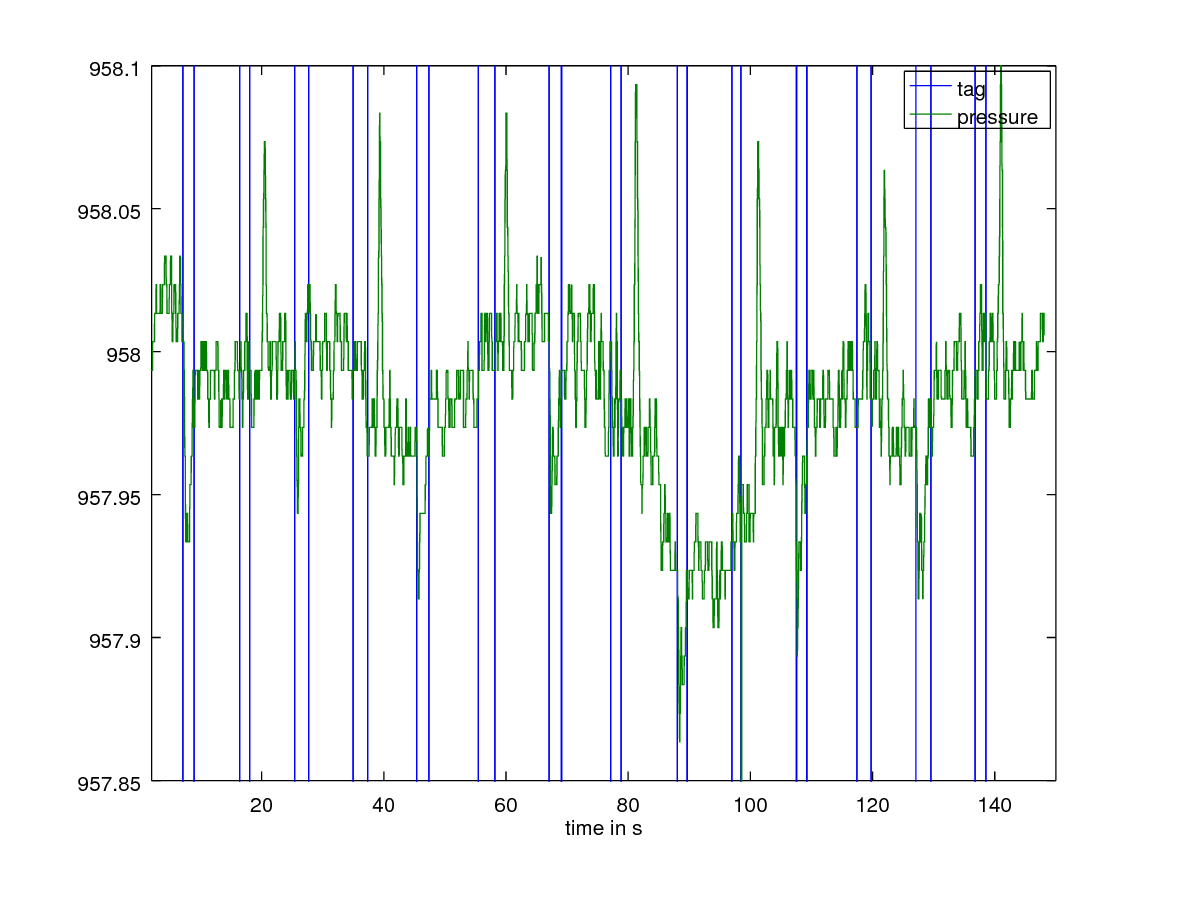
\includegraphics[width=.45\textwidth]{solmultiple778_p} &
		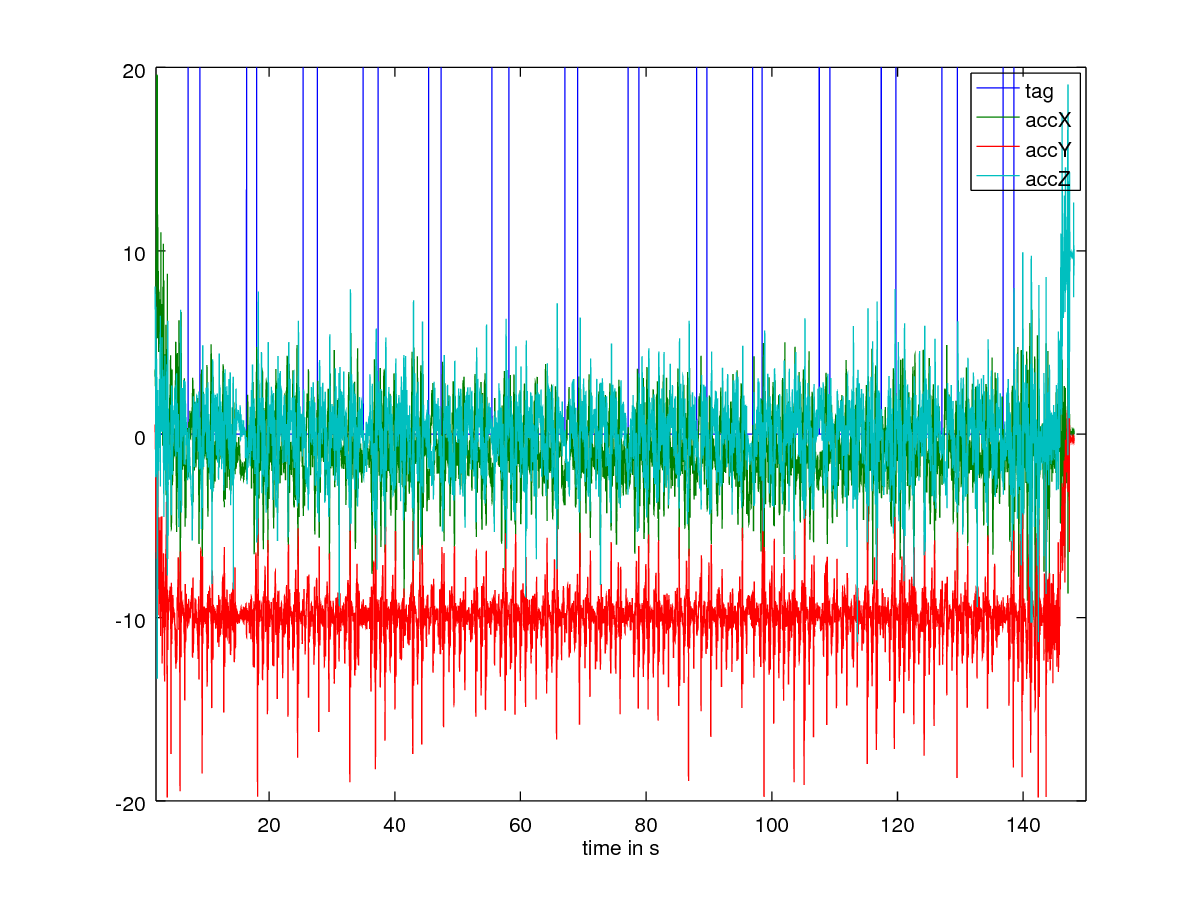
\includegraphics[width=.45\textwidth]{solmultiple778_a} 
		\\
		(a) & (b)
		\\[4pt]	%vertical extra spacing (4 points)
		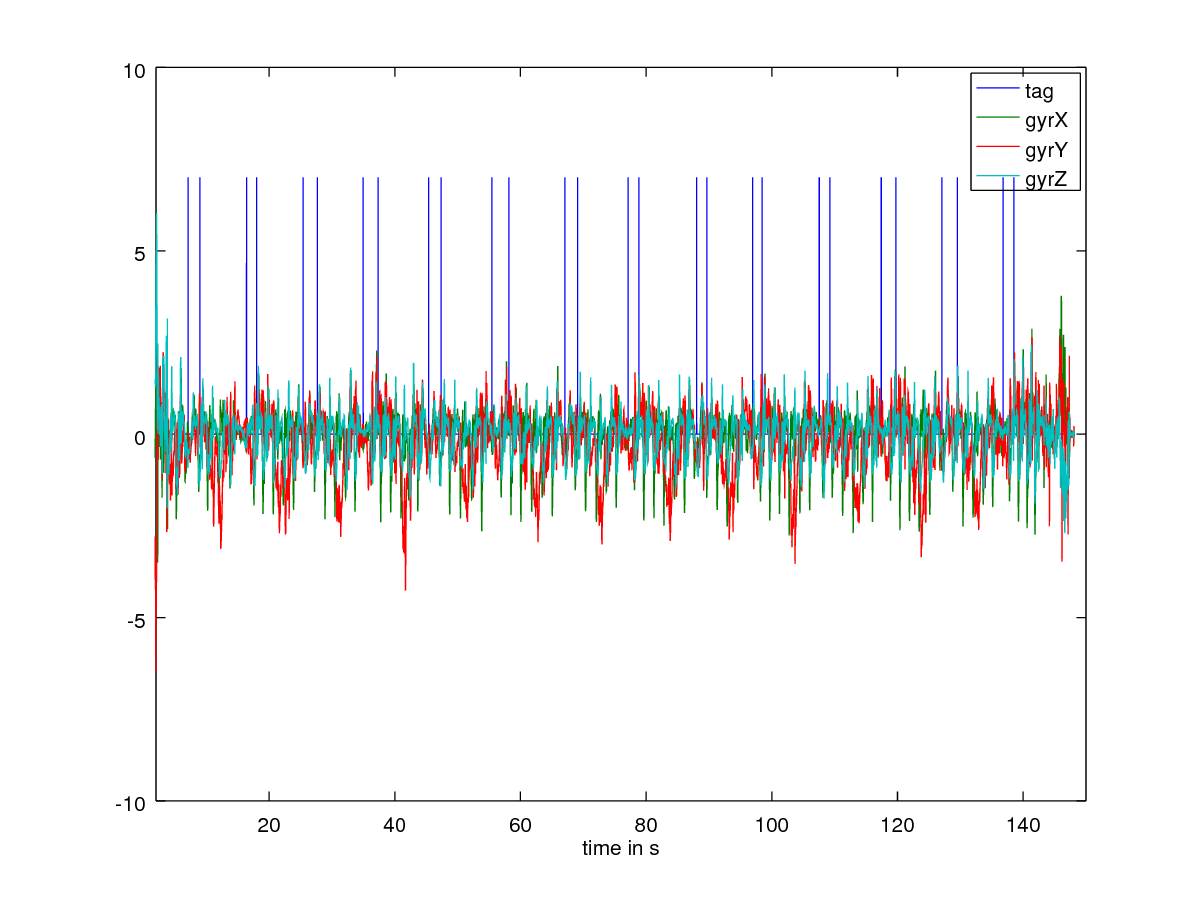
\includegraphics[width=.45\textwidth]{solmultiple778_g} &
		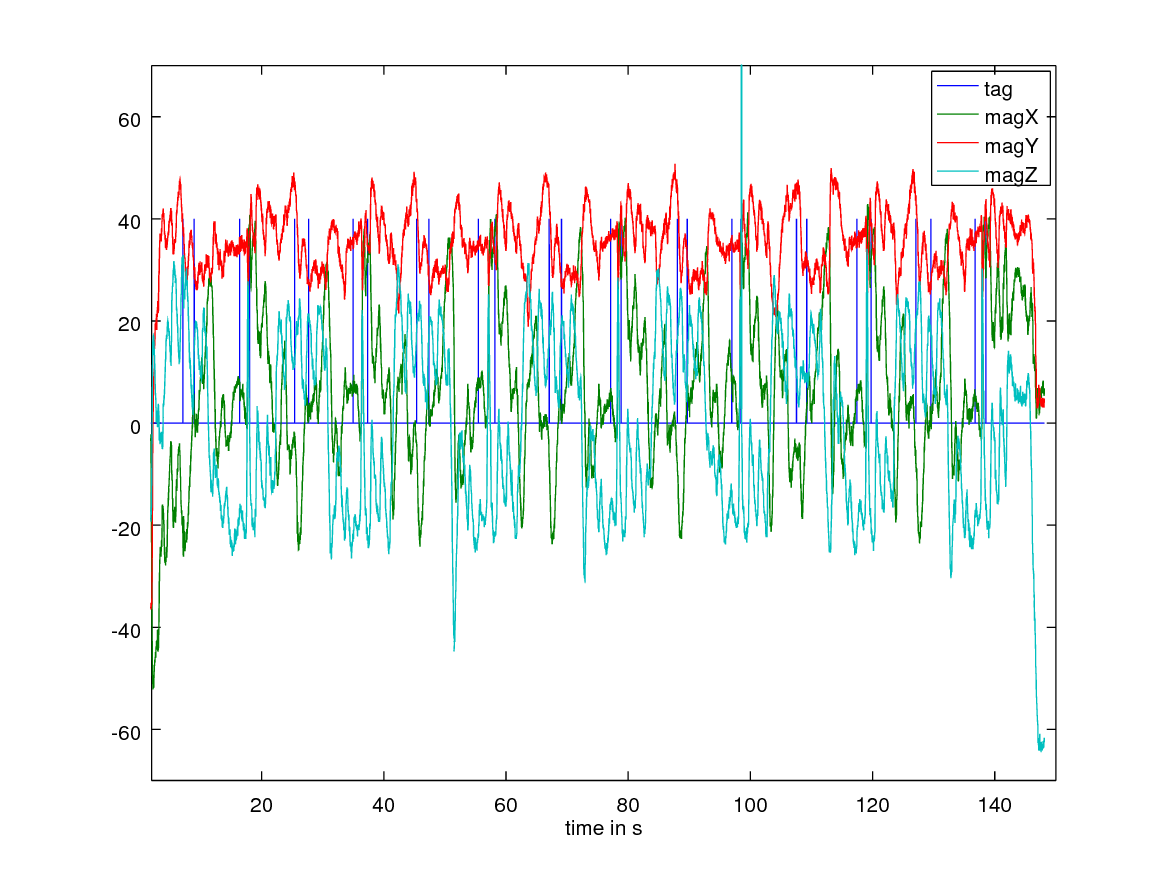
\includegraphics[width=.45\textwidth]{solmultiple778_m} 
		\\
		(c) & (d)
		\\[4pt]	%vertical extra spacing (4 points)
		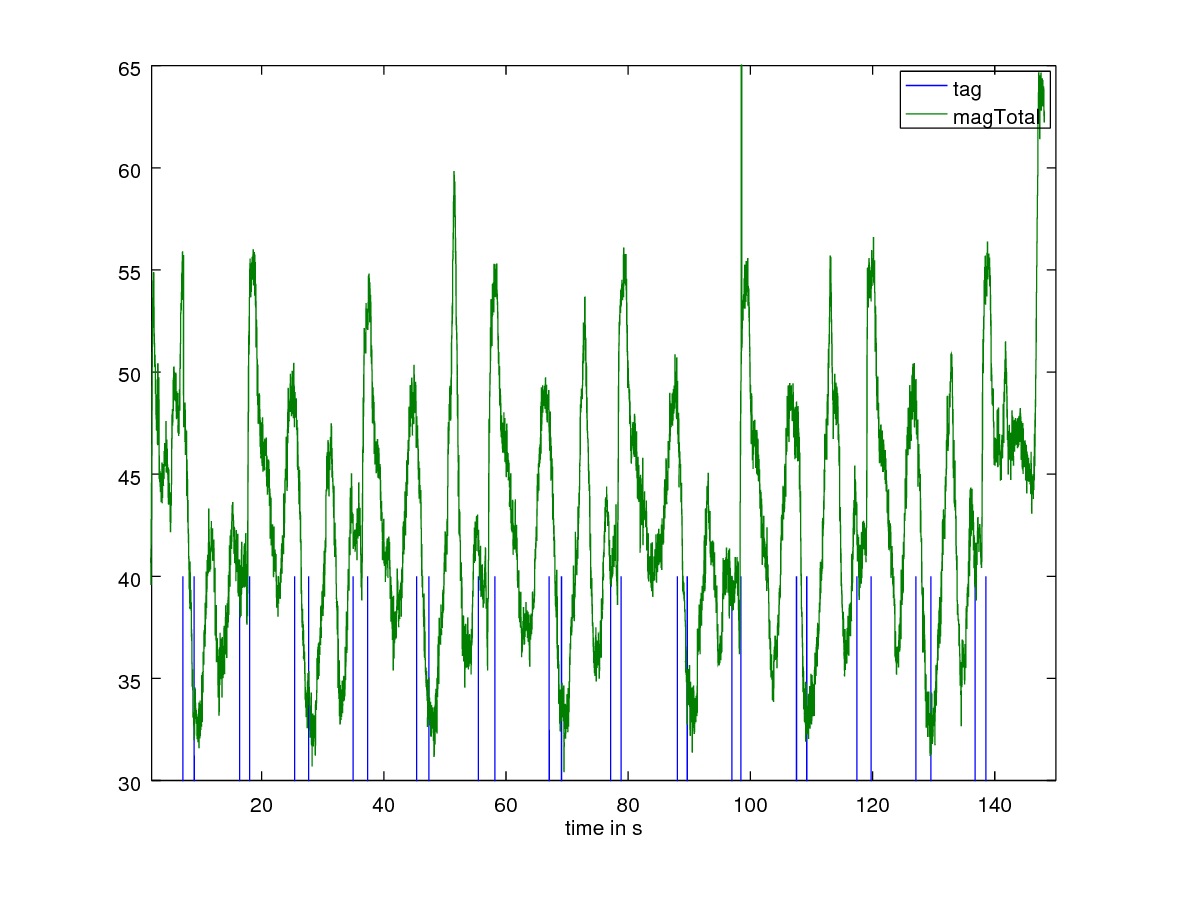
\includegraphics[width=.45\textwidth]{solmultiple778_mtotal} 
		\\
		(e)
	\end{tabular}
	%
	\caption{Test case 5}
	\label{fig:Test_case_door_5}
\end{figure}
